\documentclass{report}
\usepackage[a4paper, total={7.5in, 10in}]{geometry}
\usepackage{polski}
\usepackage[utf8]{inputenc}
\usepackage{amsmath}
\usepackage{amssymb}
\usepackage{graphicx}
\usepackage{float}
\usepackage{amsfonts}
\usepackage{sectsty}
\usepackage{titlesec}
\usepackage{setspace}
\usepackage{booktabs}
\usepackage{stix}
\usepackage{fancyhdr}
\usepackage{hyperref}
\usepackage{caption}

\usepackage{enumitem}
\usepackage{pgfplots}
\usepackage{etoolbox}
\usepackage{subcaption}
\usepackage{multirow}
\usepackage{xcolor}
\usepackage{enumitem}
\graphicspath{ {zdj} }
\pagestyle{empty}

\setlength{\parindent}{0pt}

\newcommand\setItemnumber[1]{\setcounter{enumi}{\numexpr#1-1\relax}}



\titlespacing*{\chapter}{0pt}{-35pt}{0pt}
\titlespacing*{\section}{0pt}{-20pt}{10pt}
\titlespacing*{\subsection}{0pt}{-20pt}{10pt}
\titlespacing*{\subsubsection}{0pt}{0pt}{10pt}

\titleformat{\chapter}[display]{\normalfont\Large\bfseries\filcenter}{}{10pt}{\Large}
\titleformat{\section}[display]{\normalfont\large\bfseries\filcenter}{}{10pt}{\large}
\titleformat{\subsection}[display]{\normalfont\normalsize\bfseries\filcenter}{}{10pt}{\normalsize}
\titleformat{\subsubsection}[display]{\normalfont\small\bfseries}{}{10pt}{\small}

\setcounter{tocdepth}{3}
\setcounter{secnumdepth}{3}

\pagestyle{fancy}
\fancyhf{}
\fancyfoot[R]{Strona \thepage}
\renewcommand{\headrulewidth}{1pt}
\renewcommand{\footrulewidth}{1pt}
\fancypagestyle{plain}{\pagestyle{fancy}}

\fancyfoot[L]{Popławski Dawid}%
\fancyhead[R]{}%


\DeclareCaptionFormat{custom}
{%
	\textbf{#1#2}\textit{\small #3}
}
\renewcommand{\figurename}{Rys.}

\captionsetup{format=custom,%
				margin={5pt,5pt},%
				justification=centering}
\usepackage[T1]{fontenc}       % change font encoding to T1
\usepackage[framed,numbered]{matlab-prettifier}



\begin{document}
	\begin{titlepage}
		\begin{figure}[h]
			\begin{minipage}[l]{.5\textwidth}%
				
\includegraphics[width=0.3\textwidth]{pwr_logo}
			\end{minipage}%
			\begin{minipage}[r]{.5\textwidth}%
				
\includegraphics[width=1\textwidth]{wit_logo}
			\end{minipage}%
		\end{figure}
		
		\vspace*{3mm}
		
		\begin{center}
			\rule{\textwidth}{0.8pt}\\ 
			\vspace*{6mm}
			{\LARGE Platformy programistyczne .Net i Java - LAB3}\\
			\vspace*{3mm}
			\rule{\textwidth}{0.8pt}\\
			
			\vspace{1.5cm}
			{\setstretch{2}
				Politechnika Wrocławska
				
				Wydział Informatyki i telekomunikacji
				
				Kierunek: Informatyczne systemy automatyki
				
				grupa nr 2
				
				\href{https://github.com/wernexnrs/264254-.NET-i-Java}{github.com/wernexnrs/264254-.NET-i-Java}
				
			}
		\end{center}
		
		\vspace*{2cm}
		
		\begin{flushright}
			{\setstretch{2}
				Dawid Popławski - $264254$
				
				Termin zajęc: Środa godz. $17^{\underline{05}}$ - $18^{\underline{45}}$ 
				
				Prowadzący: mgr inż. Michał Jaroszczuk
				
			}
			
		\end{flushright}
		
		\vfill
		
\end{titlepage}

\tableofcontents

\chapter{Opis programu}

Zaprezentowany program demonstruje zastosowanie wielowątkowości w różnych kontekstach i poziomach abstrakcji w aplikacji Windows Forms. Główne funkcje programu obejmują równoległe przetwarzanie macierzy i operacje na obrazach, gdzie kluczowym elementem jest eksploracja wpływu wielowątkowości na wydajność obliczeń. \\

Aplikacja oferuje dwa tryby przetwarzania macierzy, które różnią się podejściem do równoległości:

\begin{itemize}
	\item LL (Low-Level Multithreading): Wykorzystuje bezpośrednie zarządzanie wątkami (System.Threading.Thread) do ręcznego podziału pracy i synchronizacji. Jest to podejście "niskopoziomowe", gdzie programista ma pełną kontrolę nad procesem tworzenia, uruchamiania i synchronizacji wątków. Ta metoda jest bardziej złożona i podatna na błędy, ale oferuje większą elastyczność.
	\begin{itemize}
		\item Praca jest podzielona równomiernie między wątki, gdzie każdy wątek otrzymuje określoną liczbę wierszy do przetworzenia. Jeśli liczba wierszy N nie dzieli się równo przez liczbę wątków, ostatni wątek przetwarza dodatkowe wiersze.
		\item Każdy wątek wykonuje mnożenie dla swojego segmentu macierzy. Dla każdego wiersza, elementy wiersza są mnożone przez każdą kolumnę drugiej macierzy, a wyniki są sumowane, aby uzyskać odpowiednie elementy macierzy wynikowej.
	\end{itemize}
	\item HL (High-Level Multithreading): Używa abstrakcji takich jak Parallel.For do automatyzacji podziału pracy i zarządzania wykonaniem. Jest to "wysokopoziomowe" podejście, które redukuje ilość wymaganego kodu i potencjalnych błędów, czyniąc program łatwiejszym w implementacji i utrzymaniu.

\end{itemize}

Funkcjonalności związane z obrazami:
\begin{itemize}
	\item Umożliwia wczytanie obrazu przez użytkownika i zastosowanie różnych filtrów: skali szarości, negatywu, progowania, oraz lustrzanego odbicia.
	\item Filtry te są stosowane równolegle za pomocą Parallel.Invoke(), co demonstruje wykorzystanie wielowątkowości do przyspieszenia operacji na obrazach.
\end{itemize}


\vspace*{15pt}
{\let\clearpage\relax\chapter{Uzyskane dane z przeprowadzonych eksperymentów}}

\begin{table}[H]
	\centering
	\begin{tabular}{|cccc|}
		\hline
		\multicolumn{4}{|c|}{\textbf{1  wątek}}                                                                                            \\ \hline
		\multicolumn{1}{|c|}{\textbf{Rozmiar macierzy}} & \multicolumn{1}{c|}{\textbf{S}} & \multicolumn{1}{c|}{\textbf{LL}} & \textbf{HL} \\ \hline
		\multicolumn{1}{|c|}{100}                       & \multicolumn{1}{c|}{0,0163}     & \multicolumn{1}{c|}{0,0175}      & 0,02        \\ \hline
		\multicolumn{1}{|c|}{150}                       & \multicolumn{1}{c|}{0,0554}     & \multicolumn{1}{c|}{0,0547}      & 0,0758      \\ \hline
		\multicolumn{1}{|c|}{200}                       & \multicolumn{1}{c|}{0,1287}     & \multicolumn{1}{c|}{0,1282}      & 0,1314      \\ \hline
		\multicolumn{1}{|c|}{250}                       & \multicolumn{1}{c|}{0,2489}     & \multicolumn{1}{c|}{0,2497}      & 0,2541      \\ \hline
		\multicolumn{1}{|c|}{300}                       & \multicolumn{1}{c|}{0,4337}     & \multicolumn{1}{c|}{0,4299}      & 0,4372      \\ \hline
		\multicolumn{1}{|c|}{500}                       & \multicolumn{1}{c|}{1,9923}     & \multicolumn{1}{c|}{1,983}       & 2,0056      \\ \hline
		\multicolumn{1}{|c|}{600}                       & \multicolumn{1}{c|}{3,5597}     & \multicolumn{1}{c|}{3,5326}      & 3,4395      \\ \hline
		\multicolumn{1}{|c|}{650}                       & \multicolumn{1}{c|}{4,3859}     & \multicolumn{1}{c|}{4,4557}      & 4,5201      \\ \hline
		\multicolumn{1}{|c|}{800}                       & \multicolumn{1}{c|}{8,3439}     & \multicolumn{2}{c|}{-}                         \\ \hline
		\multicolumn{4}{|c|}{\textbf{2 wątki}}                                                                                             \\ \hline
		\multicolumn{1}{|c|}{100}                       & \multicolumn{1}{c|}{0,0163}     & \multicolumn{1}{c|}{0,0092}      & 0,0179      \\ \hline
		\multicolumn{1}{|c|}{150}                       & \multicolumn{1}{c|}{0,0554}     & \multicolumn{1}{c|}{0,0303}      & 0,0371      \\ \hline
		\multicolumn{1}{|c|}{200}                       & \multicolumn{1}{c|}{0,1287}     & \multicolumn{1}{c|}{0,0712}      & 0,0853      \\ \hline
		\multicolumn{1}{|c|}{250}                       & \multicolumn{1}{c|}{0,2489}     & \multicolumn{1}{c|}{0,1403}      & 0,1516      \\ \hline
		\multicolumn{1}{|c|}{300}                       & \multicolumn{1}{c|}{0,4337}     & \multicolumn{1}{c|}{0,2383}      & 0,2517      \\ \hline
		\multicolumn{1}{|c|}{500}                       & \multicolumn{1}{c|}{1,9923}     & \multicolumn{1}{c|}{1,1377}      & 1,1543      \\ \hline
		\multicolumn{1}{|c|}{600}                       & \multicolumn{1}{c|}{3,5597}     & \multicolumn{1}{c|}{1,9831}      & 2,0195      \\ \hline
		\multicolumn{1}{|c|}{650}                       & \multicolumn{1}{c|}{4,3859}     & \multicolumn{1}{c|}{2,4186}      & 2,4957      \\ \hline
		\multicolumn{1}{|c|}{800}                       & \multicolumn{1}{c|}{8,3439}     & \multicolumn{1}{c|}{4,6448}      & 4,7193      \\ \hline
		\multicolumn{4}{|c|}{\textbf{3 wątki}}                                                                                             \\ \hline
		\multicolumn{1}{|c|}{100}                       & \multicolumn{1}{c|}{0,0163}     & \multicolumn{1}{c|}{0,007}       & 0,0192      \\ \hline
		\multicolumn{1}{|c|}{150}                       & \multicolumn{1}{c|}{0,0554}     & \multicolumn{1}{c|}{0,0216}      & 0,0355      \\ \hline
		\multicolumn{1}{|c|}{200}                       & \multicolumn{1}{c|}{0,1287}     & \multicolumn{1}{c|}{0,056}       & 0,0677      \\ \hline
		\multicolumn{1}{|c|}{250}                       & \multicolumn{1}{c|}{0,2489}     & \multicolumn{1}{c|}{0,1026}      & 0,1182      \\ \hline
		\multicolumn{1}{|c|}{300}                       & \multicolumn{1}{c|}{0,4337}     & \multicolumn{1}{c|}{0,1874}      & 0,1991      \\ \hline
		\multicolumn{1}{|c|}{500}                       & \multicolumn{1}{c|}{1,9923}     & \multicolumn{1}{c|}{0,8223}      & 0,8513      \\ \hline
		\multicolumn{1}{|c|}{600}                       & \multicolumn{1}{c|}{3,5597}     & \multicolumn{1}{c|}{1,461}       & 1,5232      \\ \hline
		\multicolumn{1}{|c|}{650}                       & \multicolumn{1}{c|}{4,3859}     & \multicolumn{1}{c|}{1,7706}      & 1,8931      \\ \hline
		\multicolumn{1}{|c|}{800}                       & \multicolumn{1}{c|}{8,3439}     & \multicolumn{1}{c|}{3,3573}      & 3,4131      \\ \hline
		\multicolumn{4}{|c|}{\textbf{4 wątki}}                                                                                             \\ \hline
		\multicolumn{1}{|c|}{100}                       & \multicolumn{1}{c|}{0,0163}     & \multicolumn{1}{c|}{0,0071}      & 0,0266      \\ \hline
		\multicolumn{1}{|c|}{150}                       & \multicolumn{1}{c|}{0,0554}     & \multicolumn{1}{c|}{0,0184}      & 0,0384      \\ \hline
		\multicolumn{1}{|c|}{200}                       & \multicolumn{1}{c|}{0,1287}     & \multicolumn{1}{c|}{0,0488}      & 0,066       \\ \hline
		\multicolumn{1}{|c|}{250}                       & \multicolumn{1}{c|}{0,2489}     & \multicolumn{1}{c|}{0,0883}      & 0,1034      \\ \hline
		\multicolumn{1}{|c|}{300}                       & \multicolumn{1}{c|}{0,4337}     & \multicolumn{1}{c|}{0,1572}      & 0,1852      \\ \hline
		\multicolumn{1}{|c|}{500}                       & \multicolumn{1}{c|}{1,9923}     & \multicolumn{1}{c|}{0,7333}      & 0,7195      \\ \hline
		\multicolumn{1}{|c|}{600}                       & \multicolumn{1}{c|}{3,5597}     & \multicolumn{1}{c|}{1,2012}      & 1,3347      \\ \hline
		\multicolumn{1}{|c|}{650}                       & \multicolumn{1}{c|}{4,3859}     & \multicolumn{1}{c|}{1,5038}      & 1,574       \\ \hline
		\multicolumn{1}{|c|}{800}                       & \multicolumn{1}{c|}{8,3439}     & \multicolumn{1}{c|}{2,7907}      & 2,8952      \\ \hline
	\end{tabular}
	\caption{Tabela przedstawiająca czasy wykonywania dla poszczególbych metod z wybranymi ilościami wątków.}
\end{table}

{\let\clearpage\relax\chapter{Wykresy}}


\begin{figure}[H]%
	\centering
	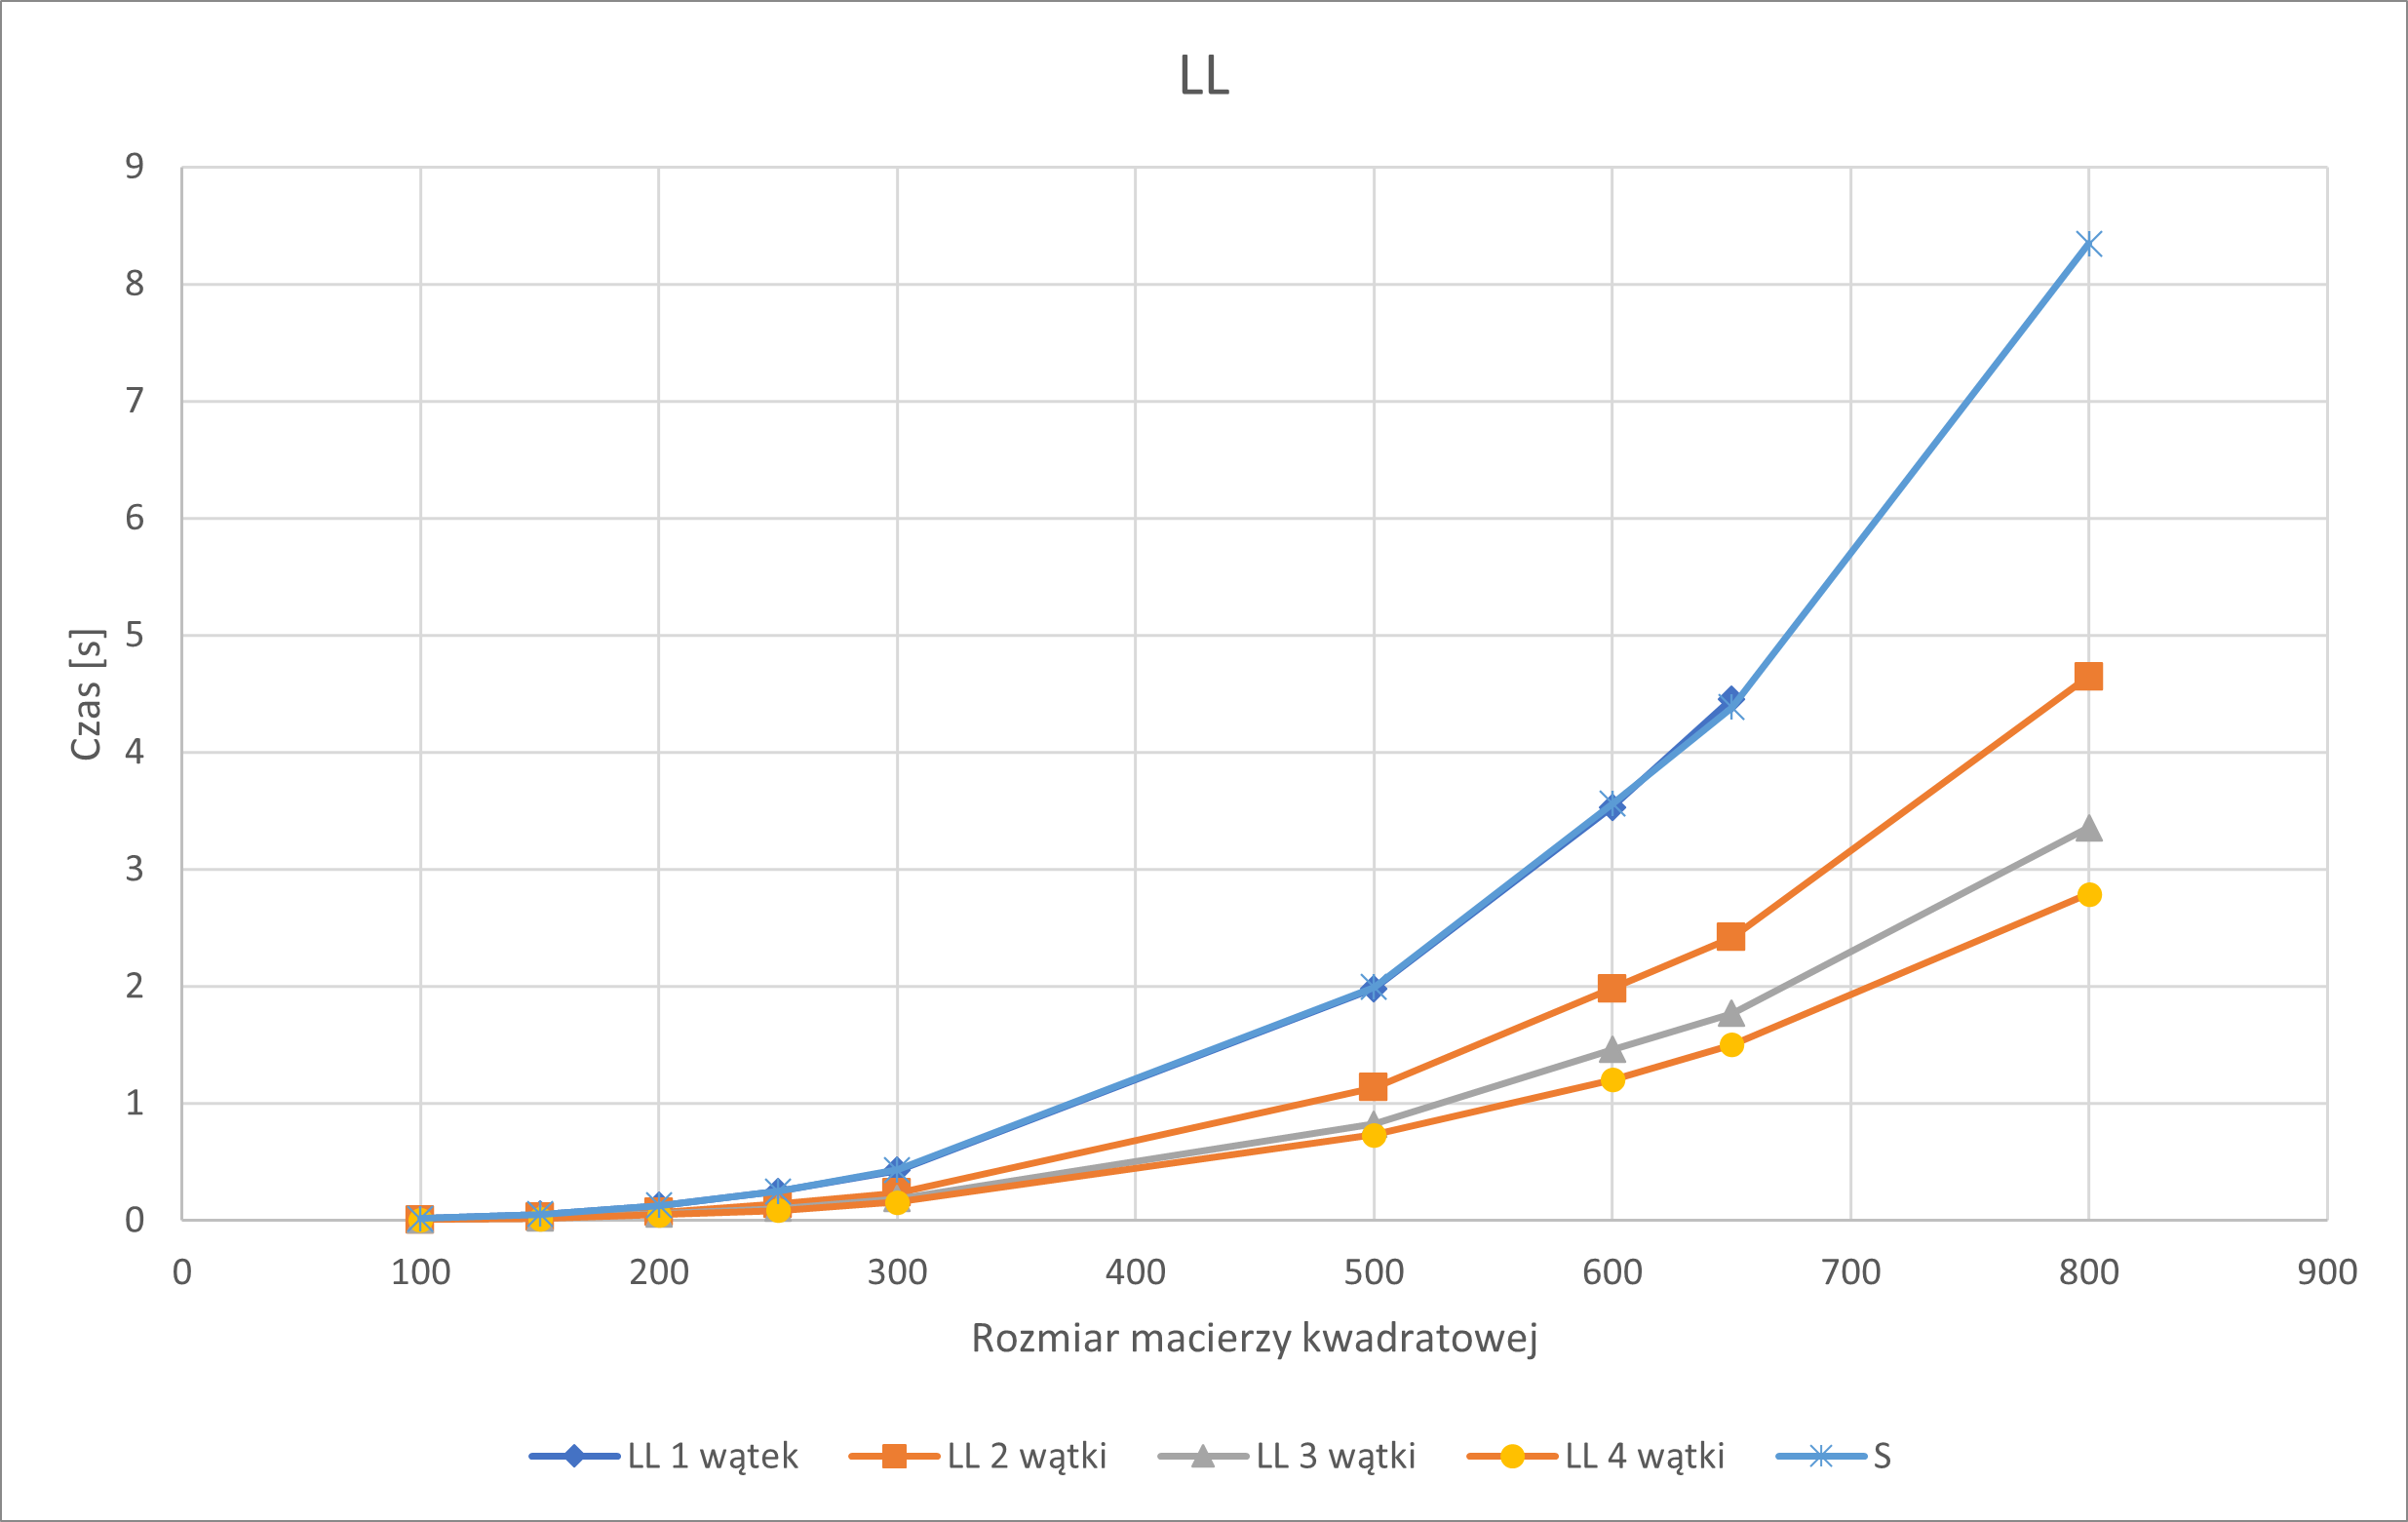
\includegraphics[scale=0.7]{zdj/LL}
	\caption{Wykres przedstawiający zależność czasu wykonanai od rozmiaru macierzy dla wielowątkowości niskiego poziomu.}
\end{figure}

\begin{figure}[H]%
	\centering
	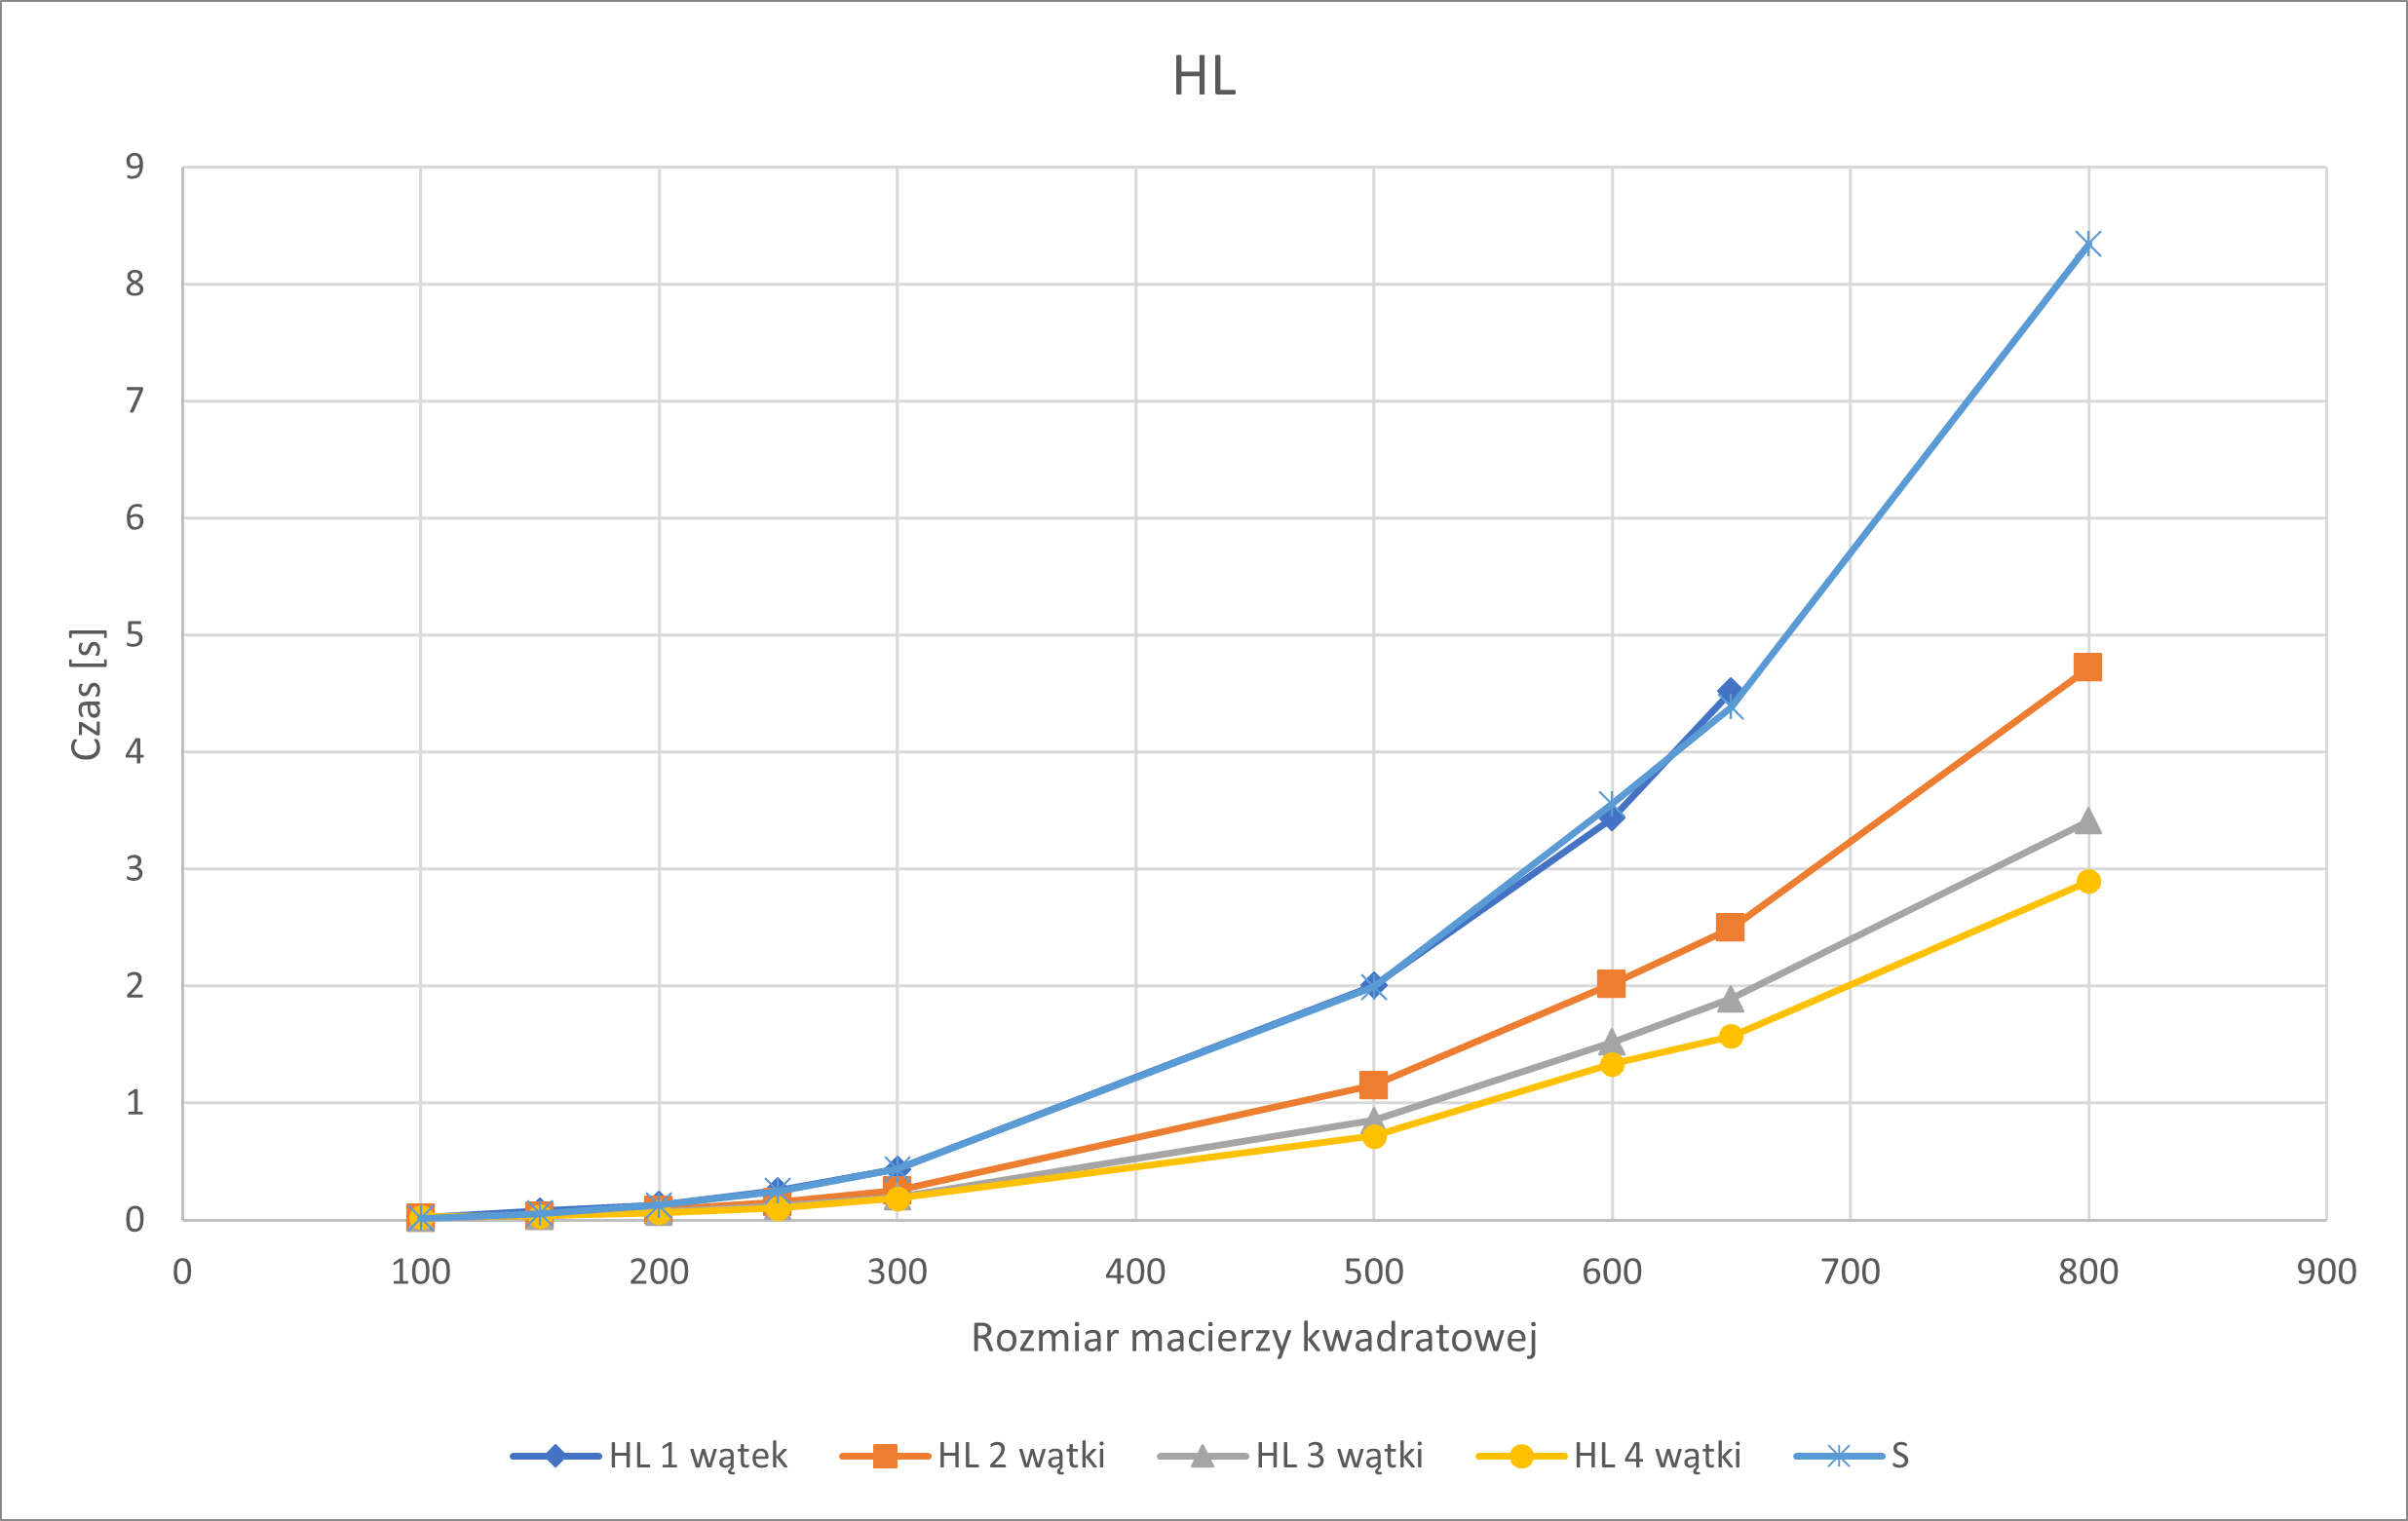
\includegraphics[scale=0.7]{zdj/HL}
	\caption{Wykres przedstawiający zależność czasu wykonanai od rozmiaru macierzy dla wielowątkowości wysokiego poziomu.}
\end{figure}

\begin{figure}[H]%
	\centering
	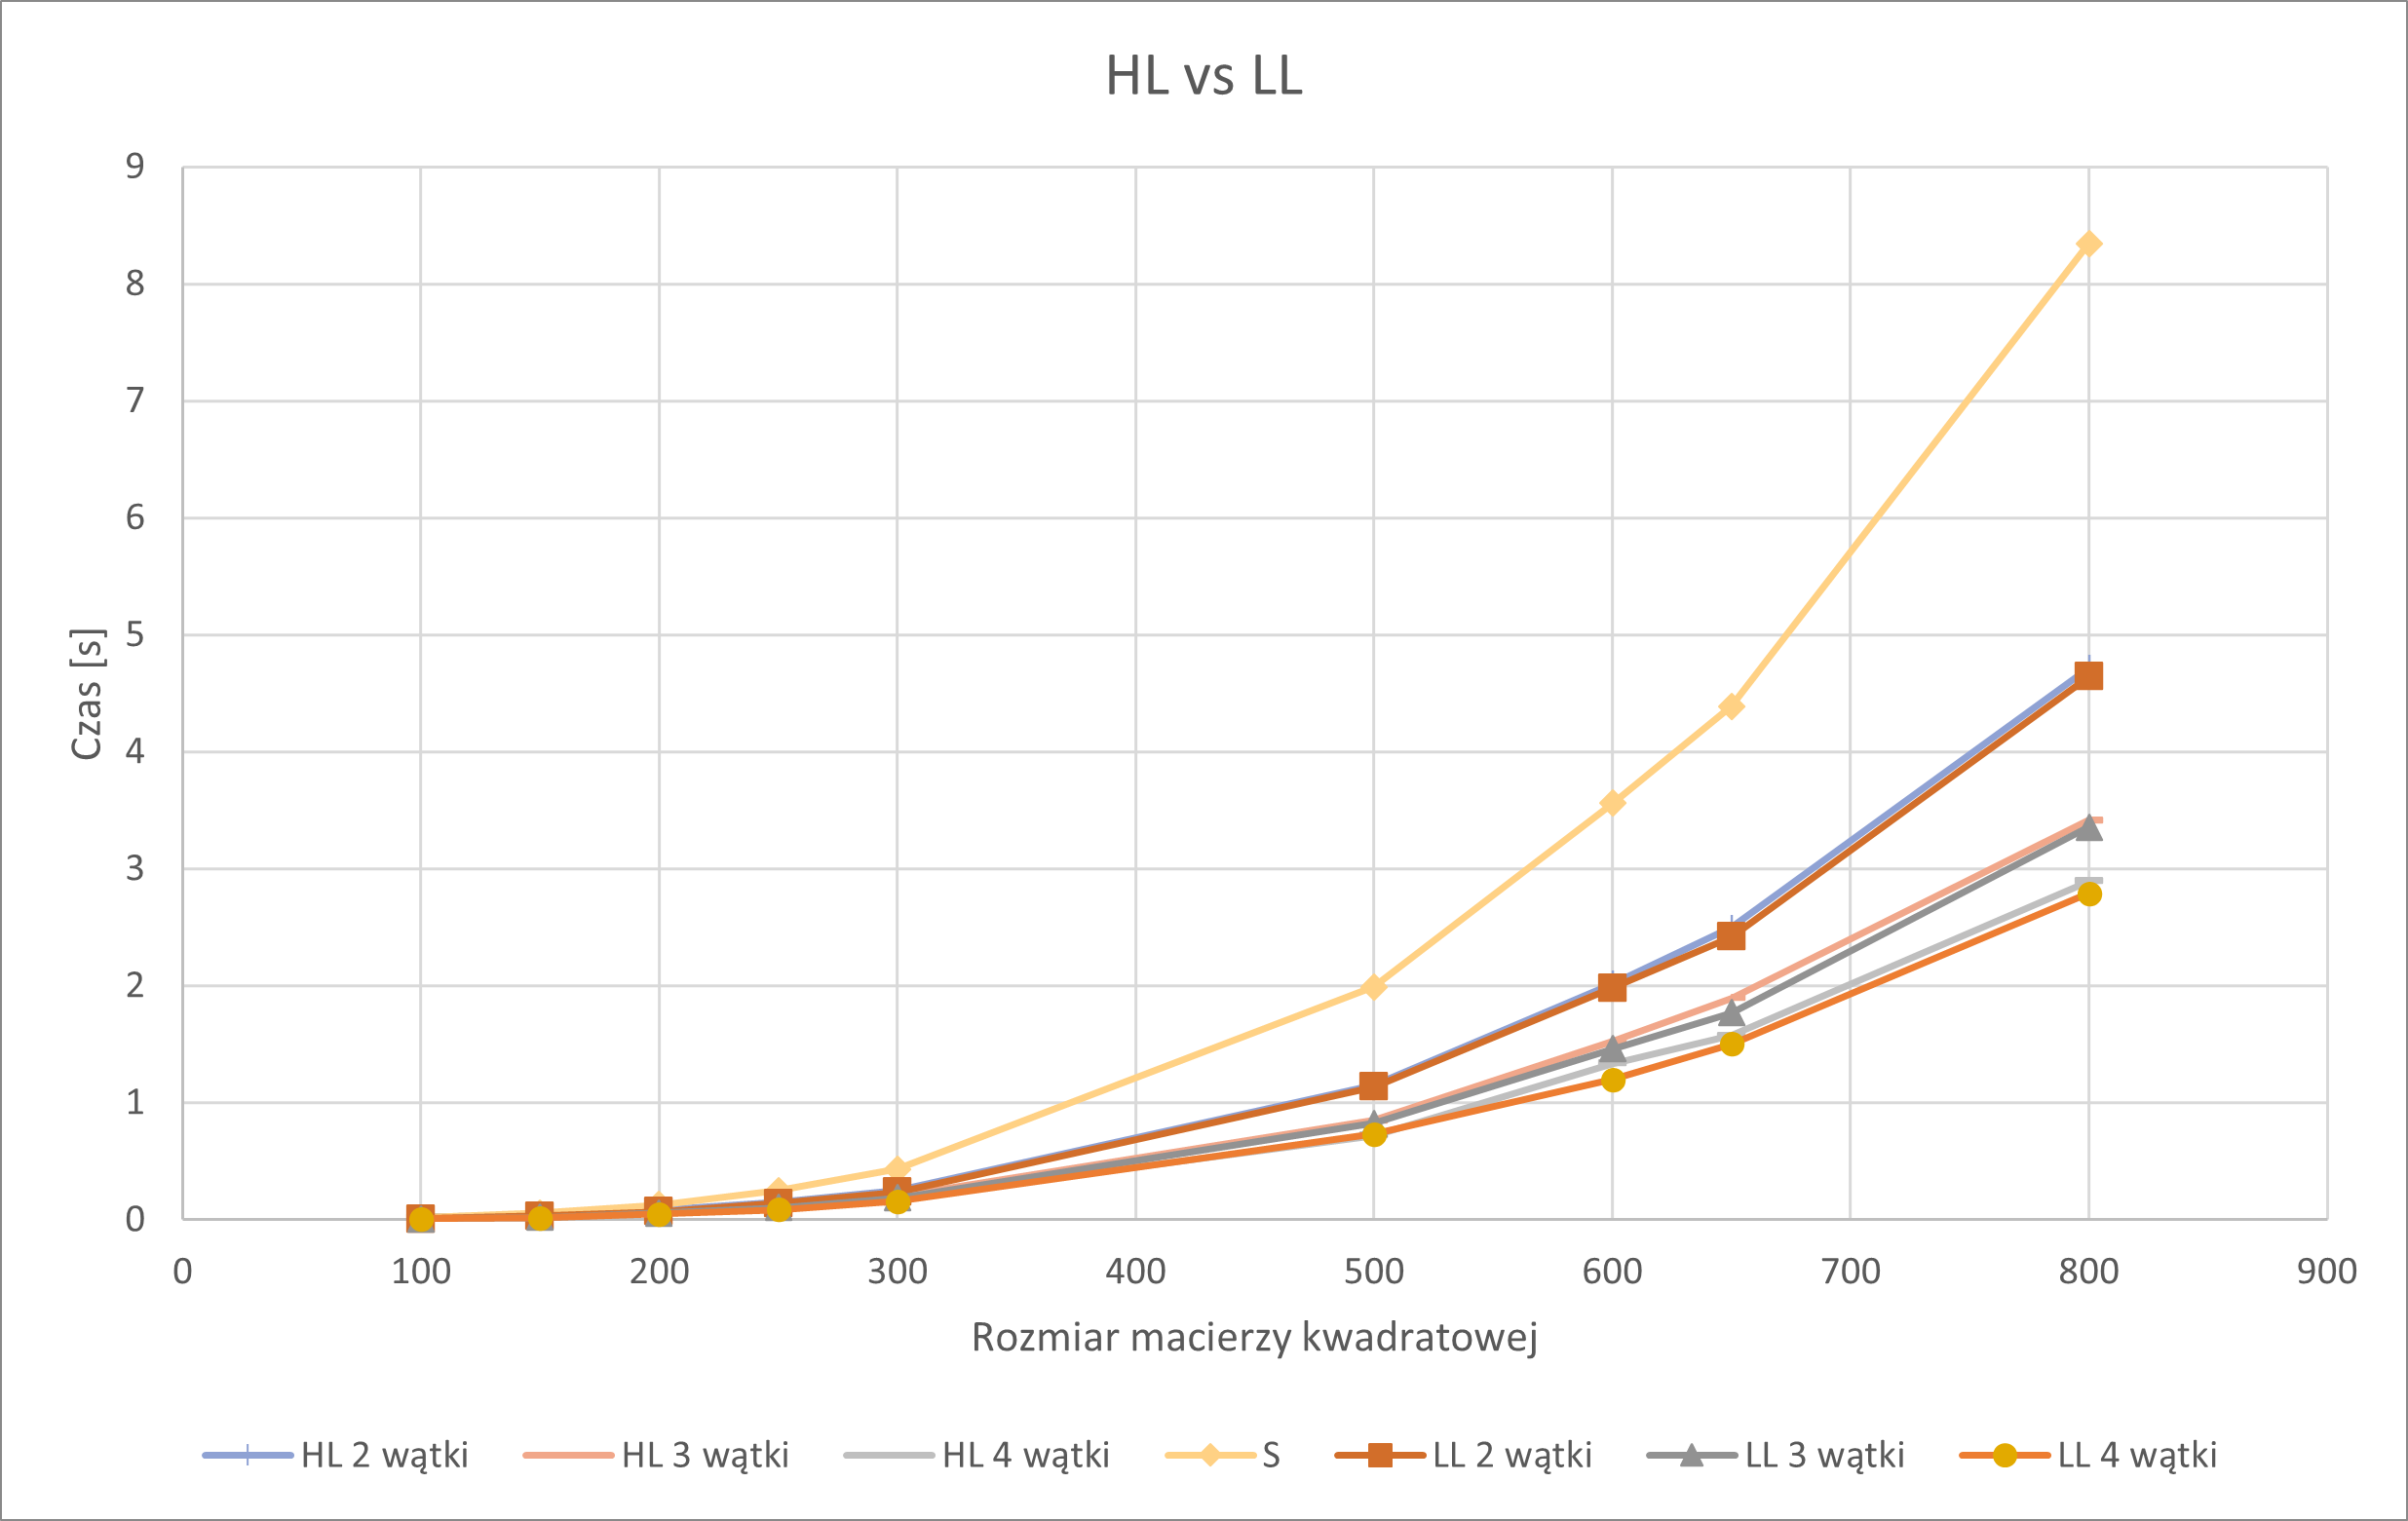
\includegraphics[scale=0.7]{zdj/both}
	\caption{Wykres przedstawiający zależność czasu wykonanai od rozmiaru macierzy dla wielowątkowości obu poziomów.}
\end{figure}

\begin{figure}[H]%
	\centering
	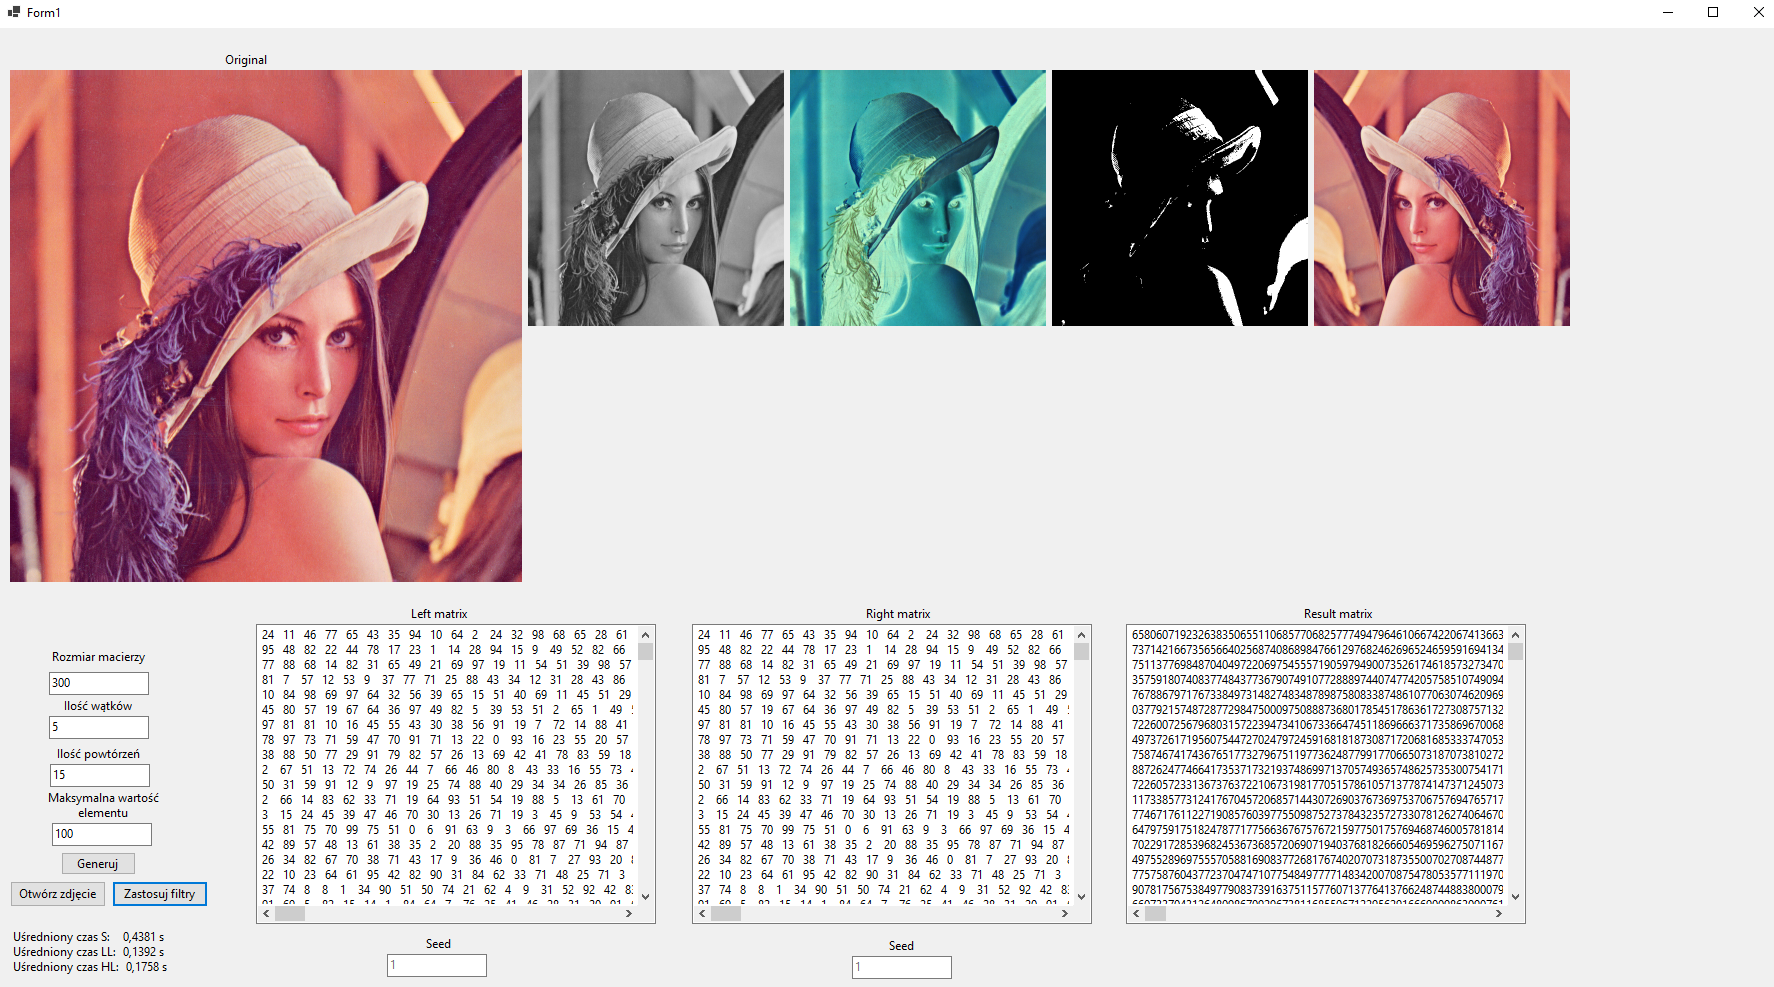
\includegraphics[scale=0.35]{zdj/main}
	\caption{Wynik programu.}
\end{figure}

\end{document}